% ---------------------------------------------------------------------------------------------------------------
\documentclass[paper=a4, fontsize=12pt]{article}
\usepackage{lipsum}% http://ctan.org/pkg/lipsum
\usepackage[explicit]{titlesec}% http://ctan.org/pkg/titlesec
\usepackage[latin1]{inputenc}
\usepackage[T1]{fontenc}
\usepackage[a4paper,pdftex]{geometry}
%\usepackage[french]{babel}
\usepackage{graphicx}
\usepackage[colorlinks=true, linkcolor=blue, urlcolor=blue, citecolor=blue]{hyperref}
\usepackage{listings}
\usepackage{xcolor}
\usepackage{array}
\usepackage{bbold}
\usepackage{wrapfig}
\usepackage{pdfpages}
\usepackage{natbib}
\usepackage{subfig}
\usepackage{array,multirow}
\usepackage{float}
\usepackage{amssymb}
\usepackage{amsmath}
\usepackage{here}
\usepackage{efbox,graphicx}
\efboxsetup{linecolor=black,linewidth=0.7pt}
\usepackage{caption} % to change caption size

\captionsetup{font=small}

% ------------------------------------------------------------------------------
\definecolor{codegreen}{rgb}{0,0.6,0}
\definecolor{codegray}{rgb}{0.5,0.5,0.5}
\definecolor{codepurple}{rgb}{0.58,0,0.82}
\definecolor{backcolour}{rgb}{0.95,0.95,0.92}

\definecolor{bleu}{rgb}{0, 0, 0.65}
\definecolor{gris}{rgb}{0.86, 0.86, 0.86}
\definecolor{vert}{rgb}{0.0, 0.5, 0.0}
\newcommand{\red}{\textcolor{red}}
\newcommand{\blue}{\textcolor{bleu}}

\bibliographystyle{plainnat}

\makeatletter
  \def\vhrulefill#1{\leavevmode\leaders\hrule\@height#1\hfill \kern\z@}
\makeatother

\def\Vhrulefill{\leavevmode\leaders\hrule height 0.8ex depth \dimexpr1.4pt-0.7ex\hfill\kern0pt}
%\titleformat{\section}{\bfseries\Large}{}{-25pt}{\noindent ~ \thesection.\quad#1~~\Vhrulefill}
%\titleformat{\subsection}{\large}{}{-2pt}{\thesubsection.\quad#1~~\textcolor{gris}{\vhrulefill{6pt}}}
\titleformat{\section}{\bfseries\Large}{}{-25pt}{\noindent ~ #1~~\Vhrulefill}
\titleformat{\subsection}{\large}{}{-2pt}{#1~~\textcolor{gris}{\vhrulefill{6pt}}}
\titleformat{\subsubsection}{\bfseries\large}{}{-2pt}{#1~~}

% ------------------------------------------------------------------------------
\lstdefinestyle{mystyle}{
    backgroundcolor=\color{backcolour},   
    commentstyle=\color{codegreen},
    keywordstyle=\color{magenta},
    numberstyle=\tiny\color{codegray},
    stringstyle=\color{codepurple},
    basicstyle=\ttfamily\scriptsize,
    breakatwhitespace=false,         
    breaklines=true,                 
    captionpos=b,                    
    keepspaces=true,                 
    numbers=left,                    
    numbersep=5pt,                  
    showspaces=false,                
    showstringspaces=false,
    showtabs=false,                  
    tabsize=2,
    language=R,                     % the language of the code
}
\lstset{style=mystyle}

% ------------------------------------------------------------------------------
\newcommand{\HRule}[1]{\rule{\linewidth}{#1}} % Horizontal rule
\makeatletter % Title
\def\printtitle{{\centering \@title\par}}
\makeatother

\makeatletter % Author
\def\printauthor{{\centering \large \@author}}
\makeatother

% ------------------------------------------------------------------------------
\title{\normalsize \textsc{} %Title page subtitle}
\\[2.0cm]\HRule{0.5pt} \\
\LARGE \textbf{\uppercase{Time Series Analysis}}
\HRule{2pt} \\ [0.5cm]\vspace*{0.2cm}
\Large{\textit{Course poject}}\\
\vspace*{3.5cm}
\normalsize}

\author{Joanne ADAM\\Data ScienceTech Institut\\
\texttt{joanne.adam@edu.dsti.institute}\\}


% ------------------------------------------------------------------------------
\begin{document}
\thispagestyle{empty} \printtitle \vfill\printauthor
\newpage

% --------------------------------------------------------------------------------------------------
\section{Database}
\subsection{}
\begin{itemize}
 \item talk about the excel file...
\end{itemize}



% --------------------------------------------------------------------------------------------------
\section{Exploratory Data Analysis}

% --------------------------------------------------------------------------------------------------
\subsection{Outliers}
Figue \ref{figure_dataset} (left) presents the datasets and show several unusual down spikes that 
could be considered as outliers (\textit{e.g.} with an electricity consumption lower than 120 kW). 
These values are remplaced by the average value of electricity consumption (see figure 
\ref{figure_dataset} right and R code below). Some statistics of the dataset are presented in table 
\ref{table_dataset}.


\begin{lstlisting}[language=R]
meani = mean(as.numeric(unlist(data[1:nrow(data),"Power (kW)"])), na.rm=TRUE)
for (index in which(z[,"Power (kW)"]<120))
  {data[index,"Power (kW)"] = meani}
\end{lstlisting} 

\begin{figure}[H]
\centering
 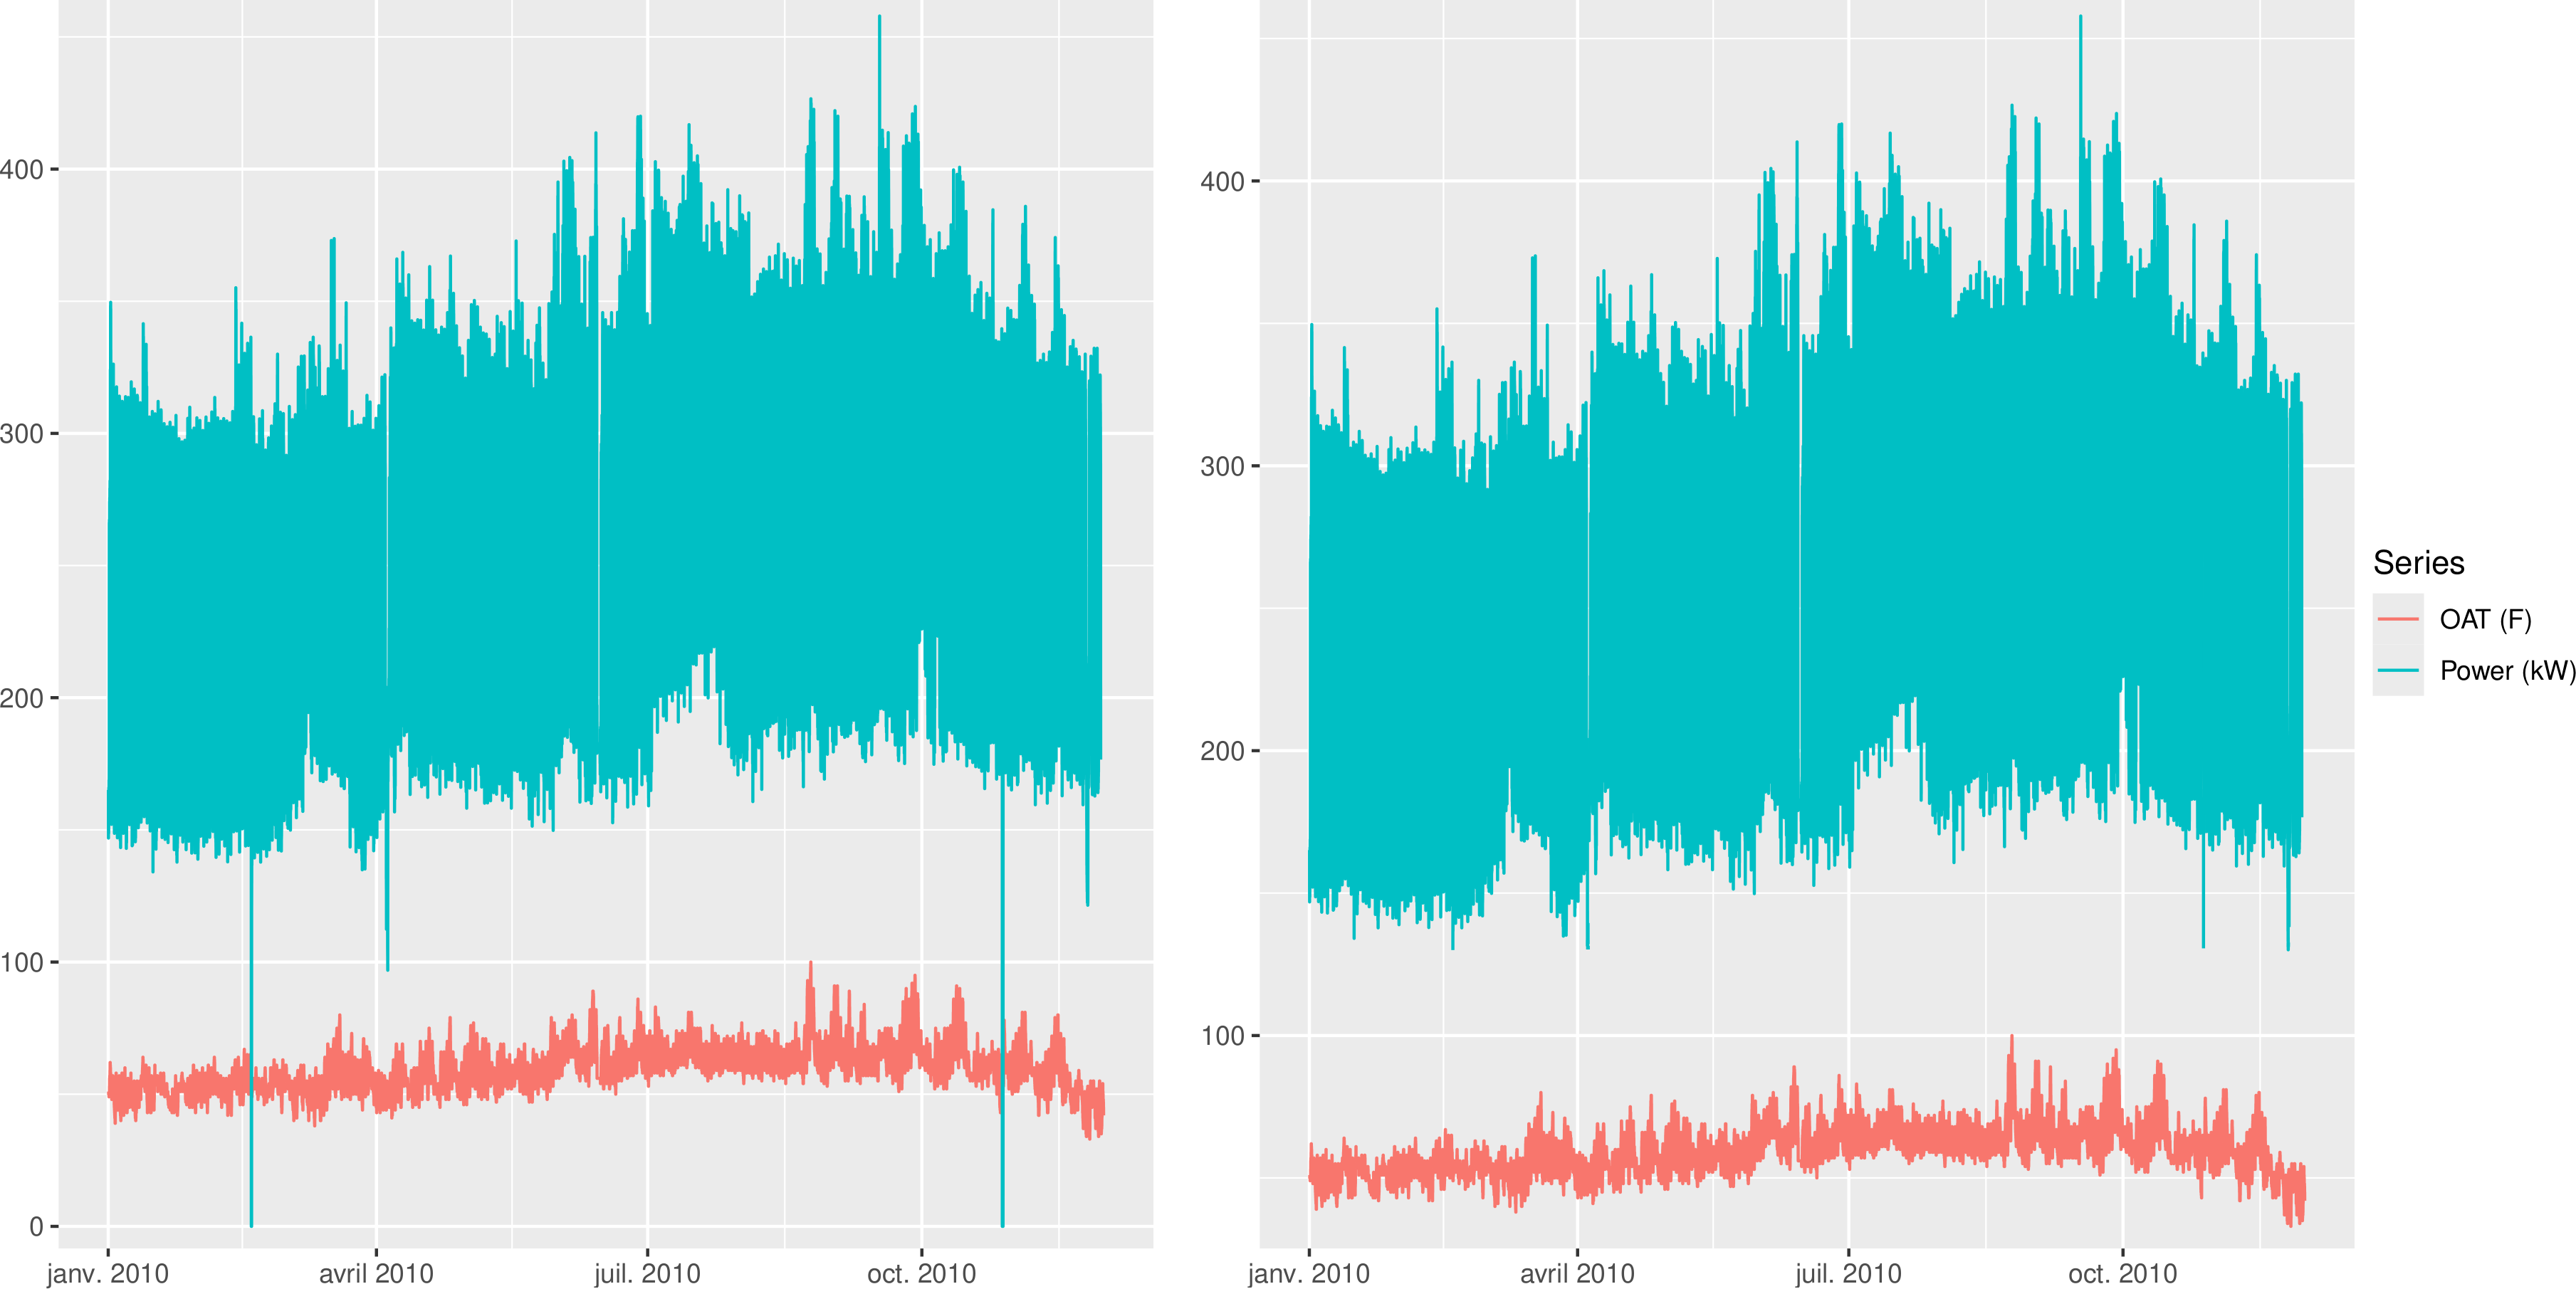
\includegraphics[scale=0.4]{figures/dataset.png}
\caption{Original dataset (left) and dataset with removed outliers (right).}
\label{figure_dataset}
\end{figure}

\begin{table}[H]
\centering \begin{tabular}{c|ccccc}
 & \textbf{Minimum} & \textbf{Maximum} & \textbf{Mean} & \textbf{Median} & \textbf{Variance} \\ \hline
\textbf{Power (kW)} &  0.0 & 457.9 & 262.3 & 276.5 & 66.0 \\
\textbf{OAT (F)}    & 33.0 & 100.0 &  59.0 &  58.0 & 8.8 \\
\end{tabular}
\caption{Basic statistics of the dataset.}
\label{table_dataset}
\end{table}


% --------------------------------------------------------------------------------------------------
\subsection{Trend and seasonality}
Using moving averages, the \texttt{decompose} R function returns the trend and seasonal components 
of the time series. Figure \ref{figure_decompose} presentes the components of the electricty power 
time series. 

\begin{figure}[H]
\centering
 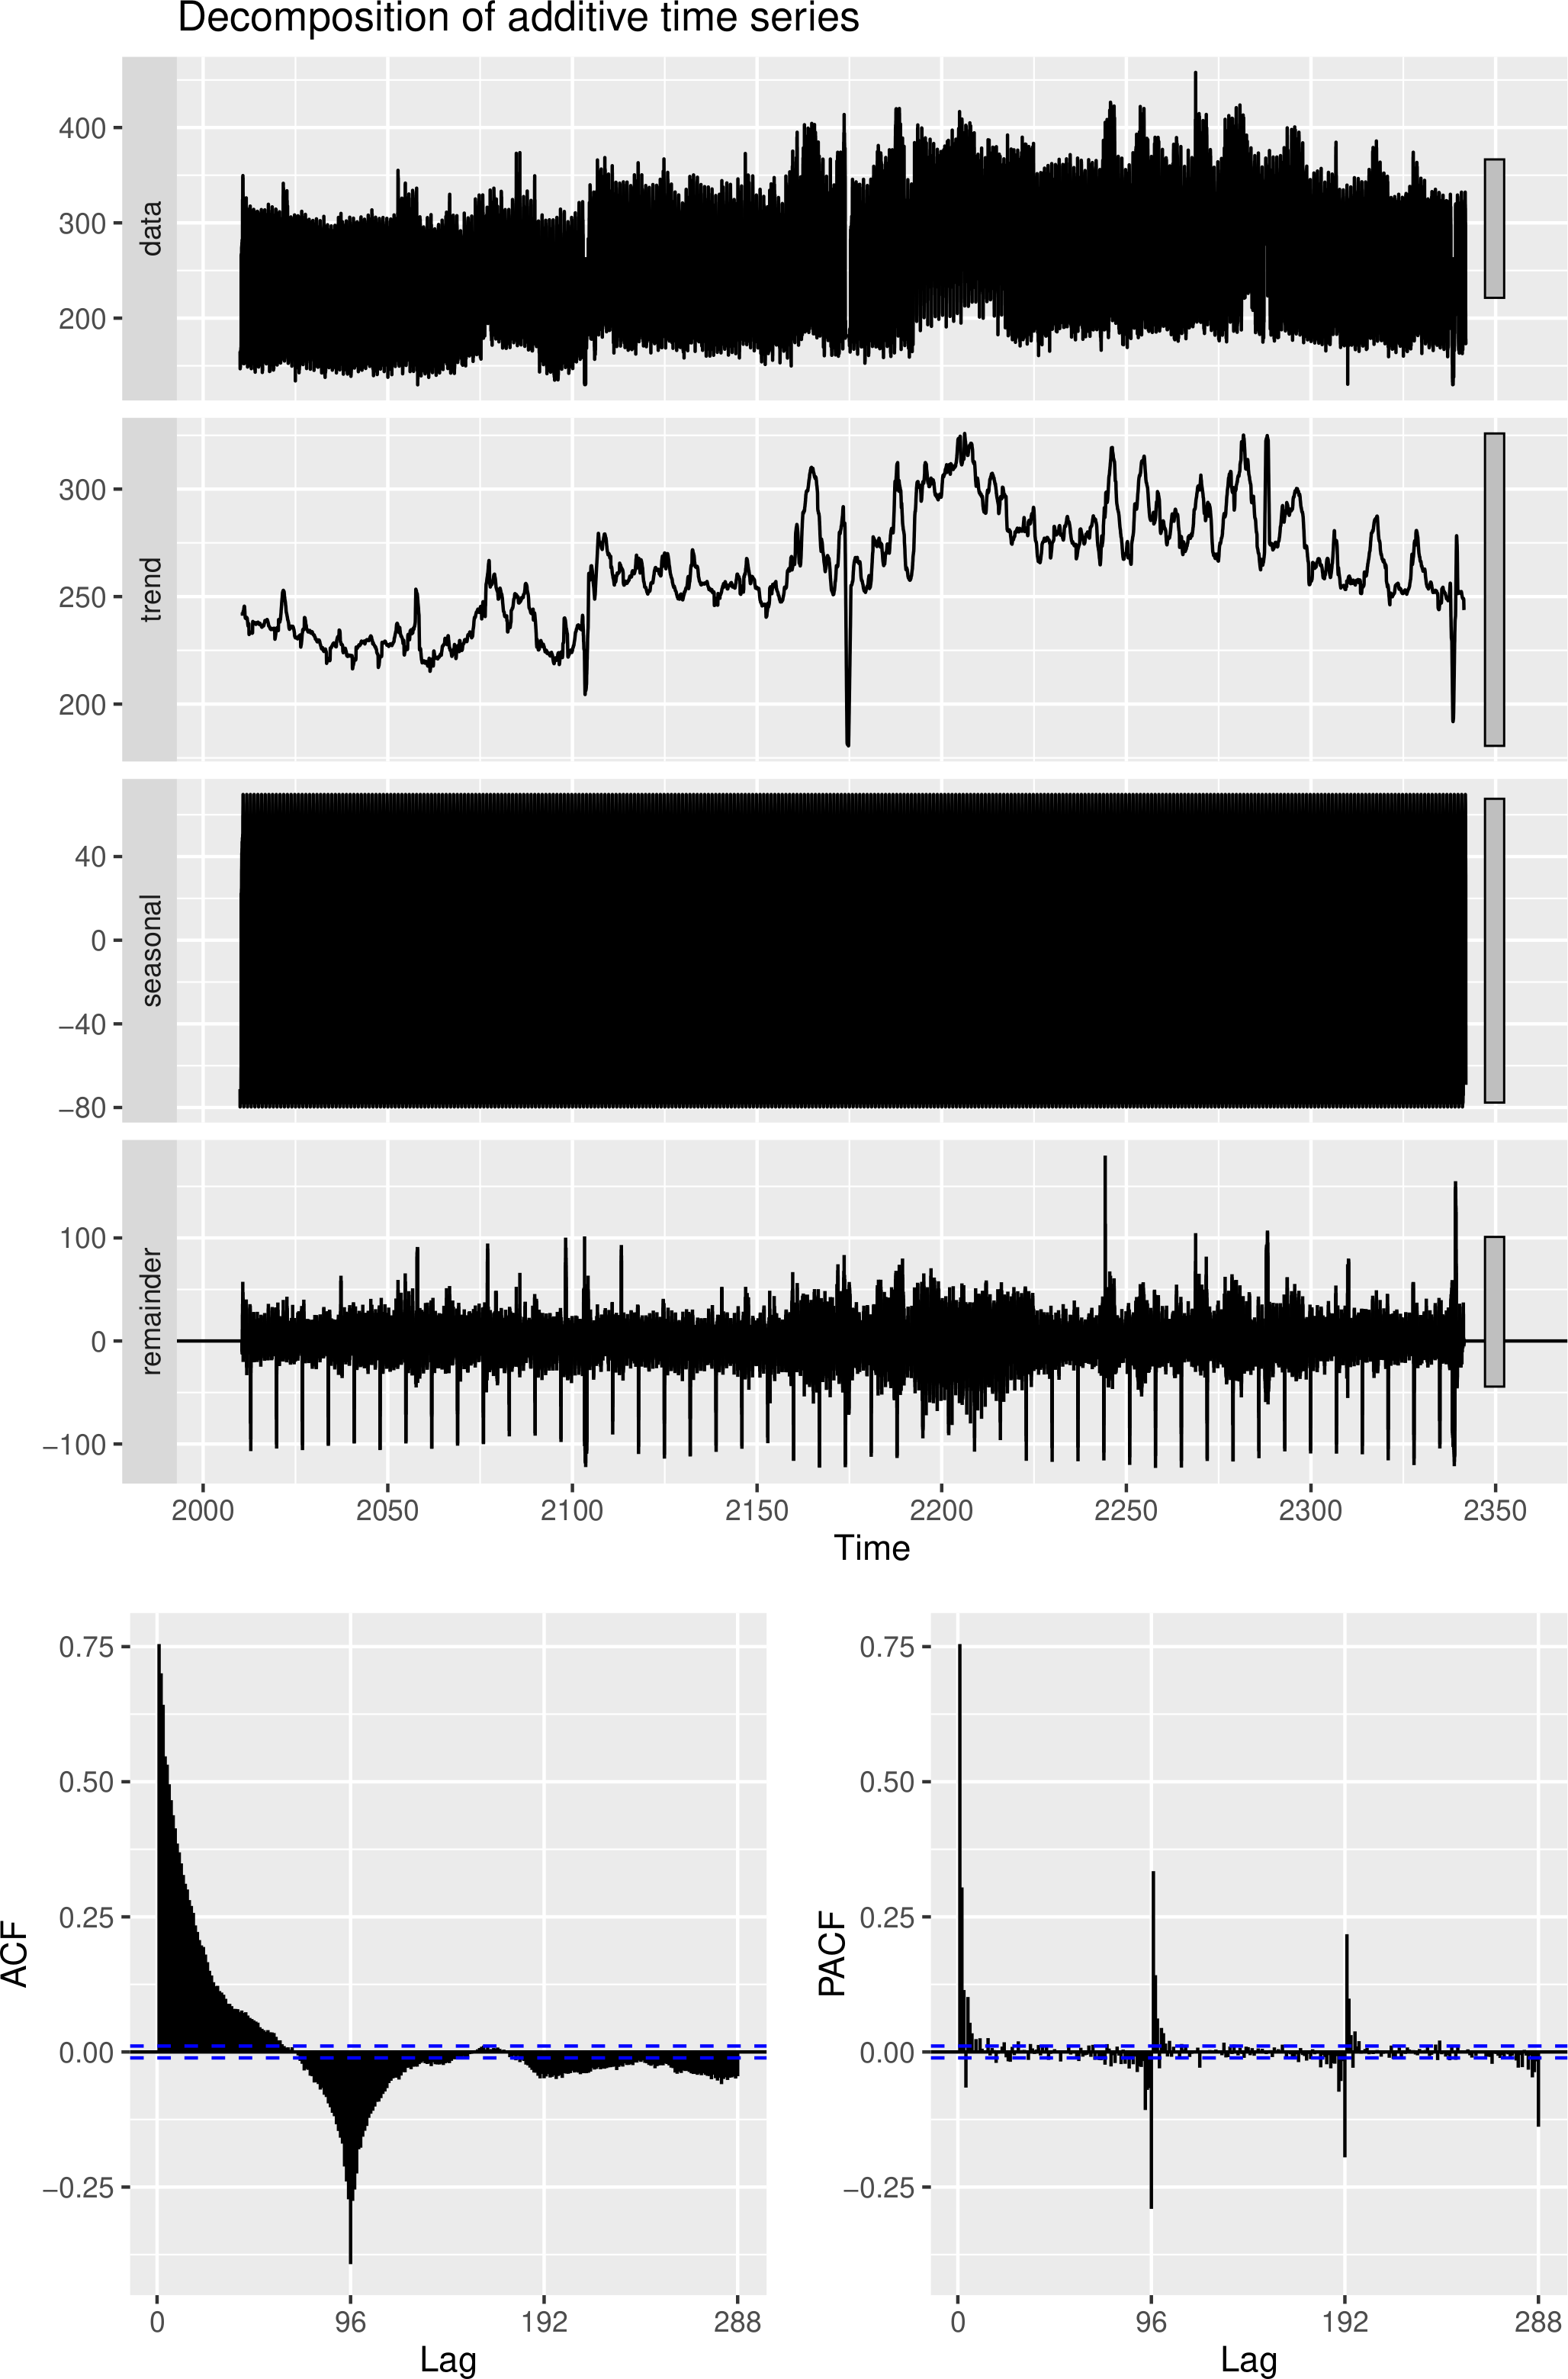
\includegraphics[scale=0.45]{figures/decompose.png}
\caption{Trend and seasonal components of the electricity consumption time series.}
\label{figure_decompose}
\end{figure}

The decomposition shows linear trend that varies in time (figure \ref{figure_decompose} TREND and 
ACF frames) and a significant seasonality of 96 lag (figure \ref{figure_decompose}, PACF frame) that 
corresponds to one day.

% --------------------------------------------------------------------------------------------------
\subsection{Noise}
The remainder of the decomposition of the electricity power time series (figure 
\ref{figure_decompose} REMAINDER frame) shows periodic fluctuations with relatively large 
amplitudes. These patterns seems to imply multi seasonality.

% --------------------------------------------------------------------------------------------------
\subsection{Covariate}
The cross-correlation test (see R code below) that test the zero-correlation between the 
electricity power time series and the covariate Outdoor Air Temperature show p-values always null. 
We reject the null hypothesis, there is no zero correlation. In other words, there is high 
correlation between the two variables. Because of this high correlation, the covariate data might 
no convey additional information. Using covariates for modelling and forecasting might not be 
significant. In this analysis modelling and forecasting is done with and without the covariate for 
comparison.

\begin{lstlisting}[language=R]
cc.test(data[,"OAT (F)"], data[,"Power (kW)"], max.lag=10, plot=FALSE) 
\end{lstlisting}

% --------------------------------------------------------------------------------------------------
\section{Modelling}
\red{\begin{itemize}
 \item Check linearity, seasonality
 \item Holt-Winters : not good method for this high frequency dataset
\end{itemize}}

% --------------------------------------------------------------------------------------------------
\subsection{SARIMA}

\red{\begin{itemize}
 \item results from auto.arima
 \item talk about problem of time needed to compute ARIMA -> use fourier
 \item without seasonality -> very bad results !!
 \item without covariates  -> very bad results !! + show new seasons not seen in 'power' (8,12,16 hours period) -> usefull to use it ?? with fourier, we could add several periods 
 \item with covariates -> no improvements. start without to try and add at end
 \item with seasonality: very long so can not do grid-search
\end{itemize}}

% --------------------------------------------------------------------------------------------------
\section{Discussion and concluding remarks}
Table \ref{table_discussion} presents the root-mean-square-error and computation time for each of 
the models presented in this report. Results show that adding Outer-Air-Temperature covariate does 
not improve significantly the fit to the model.

Model computed using XGBoost methodology as the minimum residual error and the faster computation 
time. The forecast using this model is attached in a separate file, as the prefered model.

\begin{table}[H]
\centering \begin{tabular}{c|cc}
                                    & RMSE & Computation time\\\hline\hline
SARIMA (without covariates)         &  8.60 &  56 min \\
SARIMA (with covariates)            &  8.31 &  1h16   \\
Neural Network (without covariates) & 14.93 &  1h10   \\
Neural Network (with covariates)    & 10.29 &  40 min \\
XGBoost (without covariates)        & 7.90  &  6 min
\end{tabular}
\caption{Root mean square error (RMSE) and computation time of modelling using different algorithms.}
\label{table_discussion}
\end{table}

\begin{figure}[!h]
\centering
 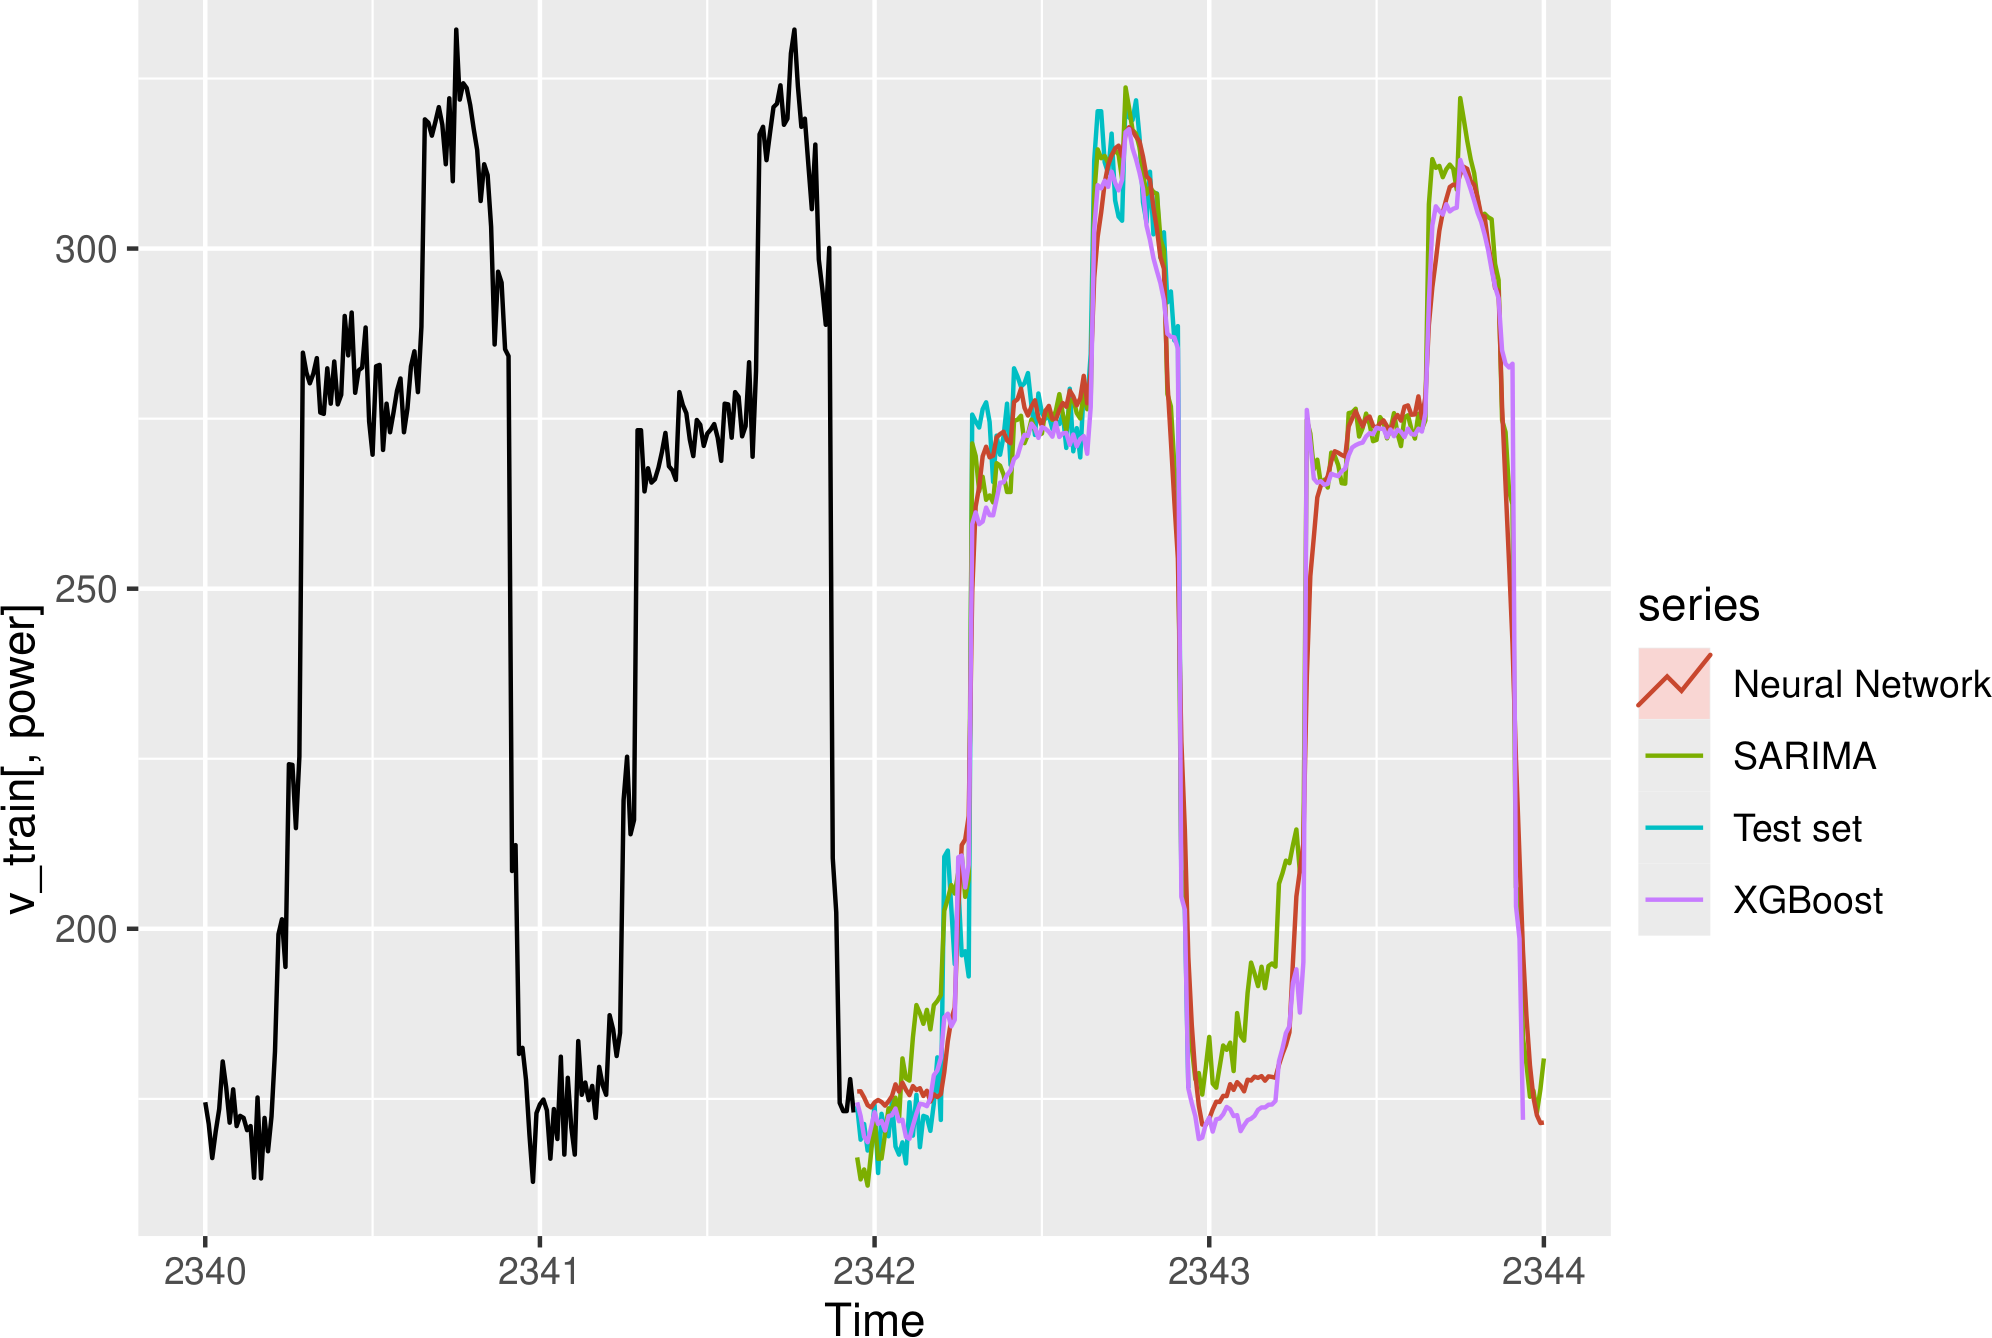
\includegraphics[scale=0.6]{figures/figure_discussion.png}
\caption{Modelling and forecast of electricity consumption using Outer-Air Temperature as a covariate.}
\label{figure_discussion}
\end{figure}

All R codes are available on Github (\url{https://github.com/JoanneAB/TimeSeriesForecasting}).



\end{document}
